%%%%%%%%%%%%%%%%%%%%%%%%%%%%%%%%%%%
%\documentclass[prd,aps,twocolumn,nofootinbib,showpacs,superscriptaddress]{revtex4-1}
\documentclass[prd,twocolumn,nofootinbib]{revtex4-1}
%\documentclass[prd,aps,nofootinbib,showpacs]{revtex4-1}
\usepackage{amsfonts}
\usepackage{amsmath}
\usepackage{amssymb}
\usepackage{bm}
\usepackage{dcolumn}
\usepackage[dvips]{graphicx}
\usepackage{graphics}
%\usepackage[latin1]{inputenc}
\usepackage{latexsym}
\usepackage{rotating}
\usepackage[colorlinks=true]{hyperref}
\usepackage{xspace} % Sensible space treatment at end of simple macros
\usepackage[usenames]{color}
\usepackage{mathrsfs}
\usepackage{multirow}
\usepackage{pifont}
\usepackage{enumitem}
\usepackage{color}
\usepackage{ulem}
\usepackage{url}
\usepackage{appendix}
\usepackage[utf8]{inputenc}
%\usepackage[toc,page]{appendix}
\usepackage{comment}
%% Try to control orphans, widows, and extra whitespace
\widowpenalty=1000
\clubpenalty=1000
\raggedbottom

\definecolor {darkgreen}{rgb}{0.2,0.7,0.2}
\definecolor{purple}{rgb}{0.5,0,0.5}

\newcommand\be{\begin{equation}}
\newcommand\ba{\begin{eqnarray}}
\newcommand\ee{\end{equation}}
\newcommand\ea{\end{eqnarray}}
\newcommand\bw{\begin{widetext}}
\newcommand\ew{\end{widetext}}
\newcommand{\lb}{\left(}
\newcommand{\rb}{\right)}

\newcommand{\EDGB}{{\mbox{\tiny EdGB}}}
\newcommand{\BD}{{\mbox{\tiny BD}}}
\newcommand{\NC}{{\mbox{\tiny NC}}}
\newcommand{\PPE}{{\mbox{\tiny PPE}}}
\newcommand{\KG}{{\mbox{\tiny kh}}}
\newcommand{\EA}{{\mbox{\tiny EA}}}
\newcommand{\ST}{{\mbox{\tiny ST}}}
\newcommand{\NS}{{\mbox{\tiny NS}}}
\newcommand{\DCS}{{\mbox{\tiny dCS}}}
\newcommand{\GR}{{\mbox{\tiny GR}}}
\newcommand{\Gdot}{{\mbox{\tiny $\dot G$}}}
\newcommand{\GW}{{\mbox{\tiny GW}}}
\newcommand{\ky}[1]{\textcolor{blue}{\it{\textbf{ky: #1}}} }
\newcommand{\kent}[1]{\textcolor{magenta}{\textbf{#1}} }
\newcommand{\st}[1]{\textcolor{cyan}{\it{\textbf{st: #1}}} }

%\bibliographystyle{apsrev}
\begin{document}
\title{Testing Gravity with Gravitational Waves from Binary Black Hole Mergers: \\ Contributions from Amplitude Corrections}

\author{Sharaban Tahura}
\affiliation{Department of Physics, University of Virginia, Charlottesville, Virginia 22904, USA.}

\author{Kent Yagi}
\affiliation{Department of Physics, University of Virginia, Charlottesville, Virginia 22904, USA.}

\author{Zack Carson}
\affiliation{Department of Physics, University of Virginia, Charlottesville, Virginia 22904, USA.}

\begin{abstract}

\ky{I've added the tentative title. We can change it later if we'd like.}

\ky{I added Zack in the author list. Somewhere in the paper, we need to show the comparison of the PPE bounds with PhenomB (that you computed) and PhenomD (that Zack computed) to justify the use of PhenomB for negative PN corrections.}

To be written later
\end{abstract}

\date{\today}




\maketitle


%%%%%%%%%%%%%%%%%%%%%%%%%%


\section{Introduction}


\section{Methodology}

In this section, we explain how we perform our analysis. We first explain the PPE formalism and non-GR waveform template. We then describe the Fisher analysis and how we construct probability distributions of non-GR parameters.

%------------------------------
\subsection{PPE Waveform}\label{section:ppE}
%Introduction
We begin by reviewing the PPE formalism briefly. PPE gravitational waveform for a compact binary inspiral in the frequency domain is given by~\cite{Yunes:2009ke}
\begin{equation}\label{eq:2a}
\tilde{h}(f)=\tilde{h}_{\GR}(1+\alpha_{\PPE}\, u^a)e^{i\delta\Psi}\,,
\end{equation}
where $\tilde{h}_{\GR}$ is the gravitational waveform in GR. $\alpha_{\PPE}\, u^a$ to the GW amplitude with $u\equiv(\pi \mathcal{M} f)^{1/3}$.  $\mathcal{M}\equiv(m_1m_2)^{3/5}/(m_1+m_2)^{1/5}$ is the chirp mass with component masses $m_1$ and $m_2$ and $f$ is the frequency of the GW. The constant $\alpha_{\PPE}$ controls the overall magnitude of the correction while the index $a$ specifies at which PN order the correction enters. One can write the non-GR phase correction $\delta\Psi$ in a similar manner as that of the amplitude as
\begin{equation}\label{eq:2b}
\delta\Psi=\beta_{\PPE} u^b\,.
\end{equation}
Together $\left(\alpha_{\PPE},a\right)$ and $\left(\beta_{\PPE},b\right)$ are called the PPE parameters.


%Parametrization
PPE modifications in Eq.~\eqref{eq:2a} can enter through the non-GR corrections to the binding energy and the GW luminosity~\cite{Yunes:2009ke,Chatziioannou:2012rf}, or alternatively to the frequency evolution and the Kepler's law~\cite{Tahura:2018zuq}. We will follow the latter approach and write the modified Kepler's law as
\begin{equation}
 \label{eq:2c}
 r=r_{\GR}(1+\gamma_r u^{c_r})\,,
 \end{equation}
and the frequency evolution as
\begin{equation}\label{eq:2d}
\dot{f}=\dot{f}_{\GR}\left(1+\gamma_{\dot{f}}u^{c_{\dot{f}}}\right)\,.
\end{equation}
Here, $\lb\gamma_r,c_r\rb$ and $\lb\gamma_{\dot{f}},c_{\dot{f}}\rb$ parametrize the non-GR corrections to the binary separation $r$ and the frequency evolution $\dot{f}$ respectively. To leading PN order, the GR contribution is given by~\cite{cutlerflanagan,Blanchet:1995ez}
\begin{equation}
r_{\GR}=\left(\frac{m}{\Omega^2}\right)^{1/3}\,, \quad
\dot{f}_{\GR}=\frac{96}{5}\pi^{8/3}\mathcal{M}^{5/3}f^{11/3}\,,
\end{equation}
where $m$ represents the total mass of the binary and $\Omega=\pi f$ is the orbital angular frequency.

%Amplitude and phase correction
Utilizing the stationary phase approximation~\cite{PhysRevD.62.084036,Yunes:2009yz} and the quadrupole formula for the metric perturbation~\cite{Blanchet:2002av}, one can easily derive the amplitude and phase of the dominant quadrupolar mode in Fourier space from Eqs.~\eqref{eq:2c} and~\eqref{eq:2d} as
\begin{equation}\label{eq:amp}
\tilde{\mathcal{A}}(f)=\tilde{\mathcal{A}}_{\GR} \left(1+2\gamma_ru^{c_r}-\frac{1}{2}\gamma_{\dot{f}}u^{c_{\dot{f}}}\right)\,,
\end{equation}
and
\be
\label{eq:Psi}
\Psi = \Psi_\GR  -\frac{15 \text{$\gamma_{\dot{f}} $}}{16 (\text{$c_{\dot{f}}$}-8) (\text{$c_{\dot{f}}$}-5)} u^{c_{\dot{f}}-5}\,,
\ee
respectively. Eq.~\eqref{eq:Psi} is already in the PPE format, while  Eq.~\eqref{eq:amp} can be reduced to such a form by keeping only the dominant correction\footnote{A detailed derivation can be found in Ref.~\cite{Tahura:2018zuq}}.\st{somewhere we have to give the definitions of dissipative and conservative corrections}


%Relation among ppE parameters
In fact, the PPE phase and the amplitude parameters may be related as follows. If the dissipative correction dominates over the conservative one, we find
\begin{equation}\label{eq:2w2}
\alpha_{\PPE} = \frac{8}{15} (a-8)(a-5) \, \beta_{\PPE}\,,
\end{equation}
while for the conservative-dominanted case, we obtains
\begin{equation}\label{eq:2w3}
\alpha_{\PPE} =\frac{8}{15} \frac{(8-a)(5-a)(a^2-4a-6)}{a^2-2a-6} \beta_{\PPE}\,.
\end{equation}
On the other hand, when the aforementioned corrections enter at the same PN order, no direct relation between $\alpha_{\PPE}$ and $\beta_{\PPE}$ exists. The exponents $a$ and $b$ in the correction terms are related by the following equation which is valid for all three cases:
\begin{equation}
b=a-5\,.
\end{equation}


%Varying-G
The above formalism needs to be slightly modified for theories containing time-varying gravitational constants. Variations in the gravitational constants cause the masses  of the binary components to vary as well~\cite{PhysRevLett.65.953}, and one needs to take this into account when deriving the PPE parameters~\cite{Tahura:2018zuq}.
%The derivation of PPE parameters for such theories can be found in Ref.~\cite{Tahura:2018zuq}






%Amplitude Correction
%Let us first derive the PPE correction to the GW amplitude. One can employ the stationary phase approximation~\cite{PhysRevD.62.084036,Yunes:2009yz} and write the amplitude of the dominant quadrupolar radiation in Fourier domain as
%\begin{equation}\label{eq:2e}
%\tilde{\mathcal{A}}(f)=\frac{A(\bar{t})}{2\sqrt{\dot{f}}}\,,
%\end{equation}
%where $A(\bar{t})$ is the GW amplitude in time domain with $\bar{t}$ representing the time corresponding to the stationary phase. $\mathcal{A}(\bar t)$ can be obtained from the quadrupole formula for the metric %perturbation~\cite{Blanchet:2002av},
% \begin{equation}\label{eq:2f}
%h^{ij}(t)\propto \frac{d^2 }{d t^2}Q^{ij}\,.
 %\end{equation}
%Here, $h^{ij}$ and $Q^{ij}$ are the $(i,j)$ components of the metric perturbation and the quadruple moment tensor respectively. For a quasi-circular binary one obtains $A(\bar{t})\propto \mu r^2f^2$ from Eq.~\eqref{eq:2f}, which after substituting to Eq.~\eqref{eq:2e} gives
%\begin{equation}\label{eq:2g}
%\tilde{\mathcal{A}}(f) \propto\frac{r^2}{\sqrt{\dot{f}}}  \,.
%\end{equation}
%Using Eq.~\eqref{eq:2c} and Eq.~\eqref{eq:2d} to Eq.~\eqref{eq:2g} one obtains, to the leading order in non-GR corrections,
%\begin{equation}\label{eq:2h}
%\tilde{\mathcal{A}}(f)=\tilde{\mathcal{A}}_{\GR} \left(1+2\gamma_ru^{c_r}-\frac{1}{2}\gamma_{\dot{f}}u^{c_{\dot{f}}}\right)\,.
%\end{equation}
%Here $\tilde{\mathcal{A}}_{\GR} $ is the amplitude of the Fourier waveform in GR. Comparing Eq.~\eqref{eq:2g} with Eq.~\eqref{eq:2a} one can read off the PPE amplitude parameters for three different cases in the following way:
%\begin{itemize}

%\item
%\emph{Dissipative-dominated Case:}
%When dissipative corrections dominate, non-GR corrections to the binary separation is negligible and one can set $\gamma_{r} = 0$. Then the PPE parameters are given by
%\begin{equation}\label{eq:2t}
%\alpha_{\PPE}=-\frac{\gamma_{\dot{f}}}{2},\quad a=c_{\dot{f}}\,.
%\end{equation}

%\item
%\emph{Conservative-dominated Case}
%When conservative corrections dominate, $c_r = c_{\dot f}$ and there is an explicit relation between $\gamma_{r}$ and $\gamma_{\dot f}$. Though finding such a relation is quite involved and one needs to go back to the original PPE formalism as explained in App.~\ref{appendix}. Non-GR corrections to the GW amplitude in such a formalism is shown in Eq.~\eqref{eq:o}. Setting the dissipative correction to zero, one finds 
%\begin{align}\label{eq:2u}
%\alpha_{\PPE}=-\frac{\gamma_r}{a}(a^2-4a-6)\,, \quad a=c_r = c_{\dot f}\,.
%\end{align} 
%\item
%\emph{Comparable Dissipative and Conservative Case}
%When dissipative and conservative corrections enter at the same PN order, $c_r=c_{\dot{f}}$ and one finds
%\begin{equation}
%\label{eq:amp-ppE-comparable}
%\alpha_{\PPE}=2 \text{$\gamma_r $}-\frac{\text{$\gamma_{\dot{f}} $}}{2}\,, \quad a=c_{r}=c_{\dot{f}}\,.
%\end{equation}
%\end{itemize}


%-------------------
\subsection{Data Analysis Formalism}

%Fisher Analysis
%%Assumptions
We adopt a Fisher analysis~\cite{Cutler:1994ys} to estimate the statistical errors of the non-GR parameters in various theories. Such an analysis is valid for GW events with sufficiently large signal-to-noise (SNR) ratios. We make the assumptions that the detector noise is Gaussian and stationary. Let us write the detector output as
\be
s(t)=n(t)+h(t)\,,
\ee
where $n(t)$ and $h(t)$ are the noise and the GW signal respectively. Let us also define the inner product of two quantities $A(t)$ and $B(t)$ as
 \be
 \left(A|B\right)=4\Re\int_0^\infty df \frac{\tilde{A}^*(f)\tilde{B}(f)}{S_n \left( f \right)}\,.
 \ee
Here $\tilde{A}(f)$ is the Fourier component of $A$, an asterisk ($*$) superscript means the complex conjugate and $S_n\left(f\right)$ is the noise spectral density. With the above definitions, the probability distribution of the noise can be written as
 \be
P\left(n=n_0(t)\right) \propto \text{exp}\left[-\left(n_0|n_0\right)\right]\,,
\ee
and the SNR for a given signal $h(t)$ can be defined as
\be
\rho \equiv\sqrt{\left(h|h\right)}\,.
\ee
Under the assumptions of a Gaussian and stationary noise, the posterior probability distribution of binary parameters $\theta^a$ takes the following form:
\be
P\left(\theta^a|s\right) \propto p^{(0)}\left(\theta^a\right) \text{exp}\left[-\frac{1}{2} \Gamma_{ab} \Delta\theta^a\Delta \theta^b \right]\,,
\ee
where $\Delta \theta^a=\hat{\theta}^a-\theta^a$ with $\hat{\theta}^a$ being the maximum likelihood values of $\theta^a$. $p^{(0)}\left(\theta^a\right)$ gives the probability distribution of the prior information, \kent{which we take to be in a Gaussian form for simplicity}. $\Gamma_{ab}$ is called the Fisher information matrix which is defined as
\be
\Gamma_{ab}=\left(\partial_a h|\partial_b h \right)\,,
\ee
where $\partial_b\equiv \frac{\partial}{\partial \theta^b}$. One can estimate the root-mean-square of $\Delta \theta^a$ by taking the square root of the diagonal elements of the inverse Fisher matrix $\Sigma^{ab}$: 
\be
\Sigma^{ab}=\left(\tilde{\Gamma}^{-1}\right)^{ab}=\langle\Delta\theta^a\Delta \theta^b\rangle\,,
\ee
where $\tilde{\Gamma}_{ab}$ is defined by
\be
p^{(0)}\left(\theta^a\right) \text{exp}\left[-\frac{1}{2} \Gamma_{ab} \Delta\theta^a\Delta \theta^b \right]=\text{exp}\left[-\frac{1}{2} \tilde{\Gamma}_{ab} \Delta\theta^a\Delta \theta^b \right]\,.
\ee

%%binary parameters
We choose the following parameters as our variables for the Fisher analysis:
\bw
\ba\label{parameters}
\theta^a\equiv \lb \ln{\mathcal{M}_z}, \ln{\eta}, \ln{D_L}, \ln{t_0}, \chi, \phi_0, \alpha, \delta, \psi, \theta_{\text{inc}}, \beta_{\PPE}, \alpha_{\PPE} \rb\,.
\ea
\ew
Here, $\mathcal{M}_z$ is the the redshifted chirp mass and $\chi$ is the effective spin parameter~\footnote{The effective spin parameter is defined as $\chi\equiv\lb m_1 \chi_1+m_2\chi_2\rb /\lb m_1+m_2\rb$, where $\chi_A$ with $A=(1,2)$ is the dimensionless spin of the $A$th body.}. $\alpha, \delta, \psi$, and  $\theta_{\text{inc}}$ are the right ascension, declination, polarization and inclination angles respectively in the detector frame. All other parameters have the same meanings as in Sec.~\ref{section:ppE}. 
%Monte-Carlo
We perform a Monte Carlo simulation by using each set of the posterior samples released by LIGO~\cite{ligo:sample} for $(\mathcal{M}_z, \eta, D_L, \chi, \alpha, \delta$, $\theta_{\text{inc}})$, while we randomly sample the polarization angle $\psi$ and the coalescence phase $\phi_0$ in $[0,\pi]$ and $[0,2\pi]$ respectively.
%%prior on spin
We impose the prior information such that the effective spin is less than 1.

%%Detectors
We use the detector sensitivity of Advanced LIGO (aLIGO) O1 run~\cite{LIGOScientific:2018mvr} and we consider the two detectors at Hanford and Livingstone. For simplicity, we assume that the Livingstone noise spectrum is identical to that of the Hanford~\cite{Yunes:2009yz}. For Fisher integration, the minimum frequency is taken to be 20 Hz while the maximum frequency is same as the cutoff frequency above which the signal power is negligible~\cite{Ajith:2009bn}.


%The rule of compound probability
Now we are going to discuss how we achieve the probability distribution of a non-GR parameter from the output of a Fisher analysis with a Monte Carlo simulation. We set the  fiducial value of any non-GR parameter to be zero for our analysis. We perform the following integration numerically to obtain the compound probability density function~\footnote{If the distribution of a random variable $y$ depends on a parameter $x$, and if $x$ is not fixed rather a random variable, the marginal distribution of $y$ is called mixture distribution or compound probability distribution and is given by $P\left(y\right)=\int P\left(y|x\right) P\left(x\right)dx$. The underlying distribution $P\left(x\right)$ is called mixing distribution or latent distribution.~\cite{2016arXiv160204060R}} of any parameter $\xi$~:
\be
\label{eq3:1}
P\lb\xi\rb=\int P\lb \xi|\sigma_{\xi}\rb P\lb \sigma_{\xi}\rb d\sigma_{\xi}\,,
\ee
where $P\lb\xi\rb$ is the marginal (unconditional) probability density function of $\xi$. $P\lb \xi|\sigma_{\xi}\rb \propto \exp[-(\xi-\bar \xi)^2/2\sigma_{\xi}^2]$ is the conditional probability density function of $\xi$ which we assume to be a Gaussian distribution with a mean $\bar \xi$ and a standard deviation $\sigma_\xi$. $P\lb\sigma_\xi\rb$ is the probability distribution of $\sigma_\xi$ computed from the Fisher analysis for the entire posterior distribution.
%We perform the integration in Eq.~\ref{eq3:1} numerically to obtain the unconditional probability density function $P\lb\xi\rb$.


%Combining amplitude and phase corrections
Let us finish this section by explaining how we can utilize both amplitude and phase corrections to derive constraints on some theory. One can include $\alpha_{\PPE}$ and $\beta_{\PPE}$ as variables to the Fisher analysis as in Eq.~\eqref{parameters} and map them to a non-GR parameter of a theory to derive constraints from the phase and amplitude independently. We refer to such constraints as  the ``phase-only'' and ``amplitude-only'' bounds respectively. How can we achieve a single constraint that accommodates both of them? Recall the relations between the PPE parameters in Sec.~\ref{section:ppE}. One can rewrite $\alpha_{\PPE}$ in the waveform in terms of $\beta_{\PPE}$ according to Eqs.~\eqref{eq:2w2} or~\eqref{eq:2w3} and eliminate the former variable from the analysis. The bound derived from $\beta_{\PPE}$ now takes into account non-GR corrections to not only the phase but also the amplitude. We refer to such constraints as the ``phase \& amplitude combined'' bounds.

%%%%%%%%%%%%%%%%%%%%%%%%%%%%%%%%%%%%%%%%%%%%%%%%%

\section{Results in Example Theories}

We now apply our analysis to some example theories. To save computational time for our Monte-Carlo simulations, we use IMRPhenomB waveform. For corrections entering through propagation mechanisms, Ref.~\cite{Yunes:2016jcc} showed that the difference in constraints on PPE parameters between IMRPhenomB and IMRPhenomD waveforms are negligible. In App.~\ref{Appendix}, we perform a similar comparison for generation mechanism corrections using sky-averaged waveforms and show that the former is only suitable for constraining generation mechanisms that enter at negative PN orders. For this reason, we consider below massive gravity, EdGB gravity, scalar-tensor theories and varying-$G$ theories. While in Massive gravity acquires non-GR corrections through propagation mechanisms while others achieve the corrections through generation mechanisms entering at negative PN orders.



\subsection{Massive Gravity}
%Intro
The idea of introducing mass to gravitons is rather old~\cite{Fierz:1939ix} and many attempts have been made to construct a feasible theory that allows to do so~\cite{deRham:2014zqa}.  Such a theory may arise in higher-dimensional setups~\cite{Hinterbichler:2011tt} and has the potential to solve the cosmic acceleration problem~\cite{deRham:2014zqa}. Although gravitons with non-zero masses may have extra polarizations as well~\cite{dePaula:2004bc}, here we study the non-GR effects due to a massive dispersion relation only.

%such as Fierz-Pauli theory and Lorentz violating massive gravity~\cite{Fierz:1939ix,Rubakov:2008nh,Rubakov:2004eb,Dubovsky:2004sg}.


%PPE parameters
We will focus on the non-GR corrections specifically to GW phase. Gravitons with non-zero mass travel at a speed smaller than the speed of light and the non-GR effects accumulate over the distance. Modified dispersion relation for such gravitons is given by $ E^2=p^2c^2+m_g^2c^4$, where $m_g$ is the mass of the graviton while $E$ and $p$ are the energy and the momentum respectively. PPE phase parameters are~\cite{Will:1997bb}
\be
\beta=\frac{\pi^2}{\lambda_g^2}\frac{\mathcal{M}}{1+z}D\,, \qquad \text{and}\qquad b=3\,,
\ee
where
\be
D=\frac{z}{H_0\sqrt{\Omega_M+\Omega_{\Lambda}}}\left[1-\frac{z}{4}\left(\frac{3\Omega_M}{\Omega_M+\Omega_{\Lambda}} \right )+\mathcal{O}(z^2)\right]\,.
\ee
Here , $\Omega_M$ and $\Omega_\Lambda$ are the energy density of matter and dark energy respectively. $H_0$ is the Hubble constant while $z$ is the redshift of the source. $\lambda_g$ is the compton wavelength of graviton that is related to $m_g$ as $\lambda_g\equiv h/\lb m_gc\rb$, where $h$ is the Planck's constant.

\begin{figure}[htb]
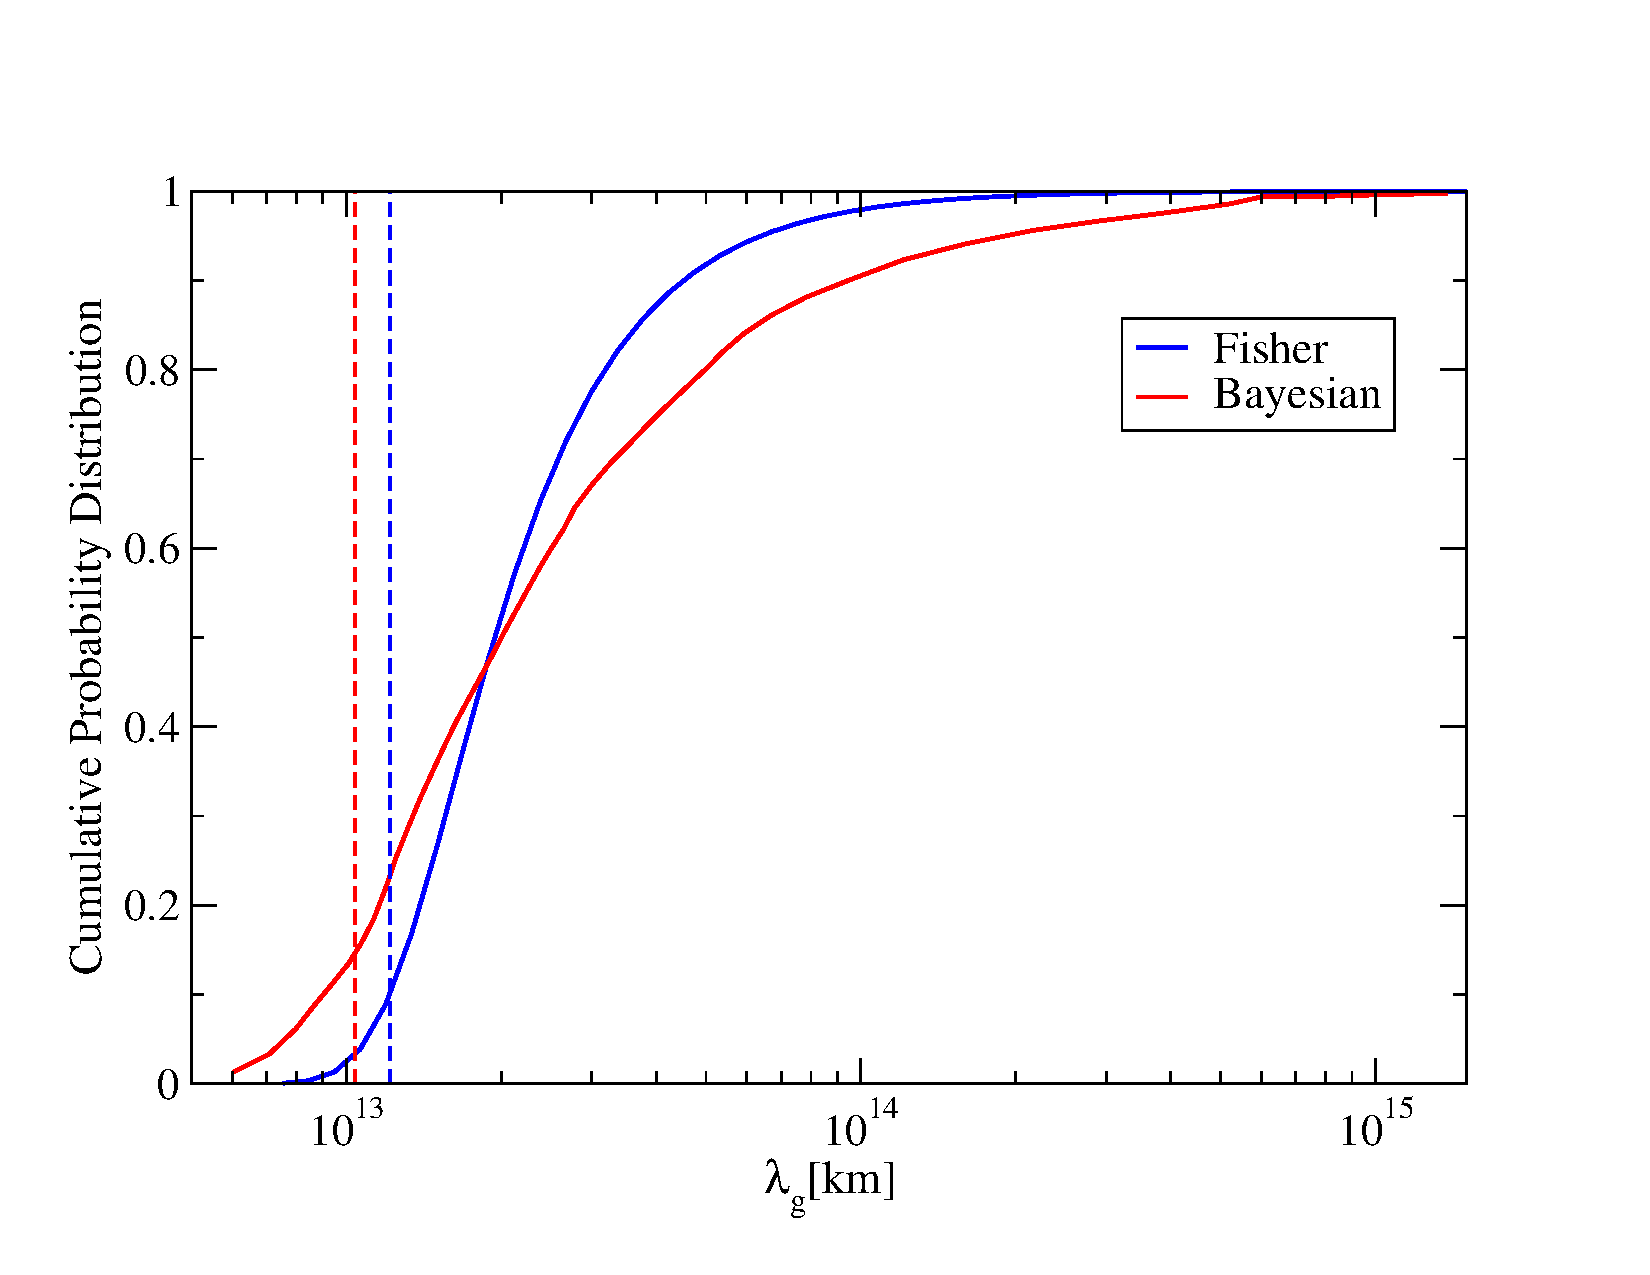
\includegraphics[width=8.5cm]{graviton.pdf}
\caption{Cumulative probability distribution of the compton wavelength of graviton from GW150914. The solid blue line is  obtained from a Fisher analysis with Monte Carlo simulation, while the red one is found by LVC via  Bayesian analysis. Each of the vertical dashed lines corresponds to the lower bound of a solid line of same color with 90\% confidence.}
\label{fig:graviton}
\end{figure}

%Result
We compute the probability distribution of $\lambda_g$ from GW150914 according to the procedure outlined in Sec.~\ref{section:ppE} and compare with the one obtained by the LVC~\cite{TheLIGOScientific:2016src} (see Fig.~\ref{fig:graviton}). The Fisher analysis with Monte Carlo simulation yields $\lambda_g<1.2\times 10^{13}$ km at 90\% CL which is in well agreement with the LVC bound of $1.04\times10^{13}$ km. The difference in the two cumulative distributions of $\lambda_g$ presented in Fig.~\ref{fig:graviton} can be attributed to the factors that the LVC used a more accurate Baysian analysis and imposed a uniform prior on the graviton mass.
%assuming a standard \text{$\Lambda$}CDM cosmology.
The GW bounds are stronger than the current solar-system and binary pulsar constraints~\cite{Talmadge:1988qz,Will:1997bb,Finn:2001qi}, while weaker than the ones from the observations of galactic clusters~\cite{Goldhaber:1974wg}, gravitational lensing~\cite{Choudhury:2002pu}, and the absence of superradiant instability in supermassive black holes~\cite{Brito:2013wya}.

\subsection{Einstein-Dilaton-Gauss-Bonnet Gravity}
%Introduction
%%Importance
EdGB gravity endows one of the simplest high-energy modification to GR~\cite{Moura:2006pz,Pani:2009wy}. Such a theory is motivated from low-energy effective string theories and also arises as a special case of Horndeski gravity~\cite{Zhang:2017unx,Berti:2015itd}. 
%%Definition
The EdGB action is given by introducing a quadratic-curvature correction (Gauss-Bonnet invariant) to the GR action that is non-minimally coupled to a scalar field (dilaton) with a coupling constant $\bar{\alpha}_\EDGB$~\cite{Kanti:1995vq}\footnote{We use barred quantities for coupling constants in order to distinguish them from the PPE parameters.}.

%ppE parameters
In EdGB gravity, BHs acquire scalar monopole charges which may generate scalar dipole radiation if they form binaries~\cite{Yagi:2011xp,Sotiriou:2014pfa,Berti:2018cxi,Prabhu:2018aun}. Such radiation leads to an earlier coalescence of BH binaries compared to that of GR and modifies the gravitational waveform with the PPE parameters given by~\cite{Yunes:2016jcc,Yagi:2011xp}
\begin{equation}
 \beta_\EDGB=-\frac{5}{7168}\zeta_\EDGB\frac{(m_1^2\tilde s_2^\EDGB-m_2^2\tilde s_1^\EDGB)^2}{m^4\eta^{18/5}}\,,
 \end{equation}
 with $b=-7$ and 
  \begin{equation}
 \alpha_\EDGB=-\frac{5}{192}\zeta_\EDGB\frac{(m_1^2 \tilde s_2^\EDGB-m_2^2 \tilde s_1^\EDGB)^2}{m^4\eta^{18/5}}\,,
 \end{equation}
 with $a=-2$.  Here, $\zeta_\EDGB\equiv 16 \pi \bar{\alpha}_\EDGB^2/m^4$ is the dimensionless EdGB coupling parameter and $\tilde s_{A}^\EDGB$ are the spin-dependent factors of the BH scalar charges given by $\tilde s_{A}^\EDGB\equiv 2(\sqrt{1-{\chi_A}^2}-1+{\chi_A}^2)/{\chi_A}^2~$~\cite{Berti:2018cxi,Prabhu:2018aun}\footnote{For ordinary stars like NSs $\tilde s_A^\EDGB$ are zero~\cite{Yagi:2011xp,Yagi:2015oca}.}.

\begin{figure}[htb]
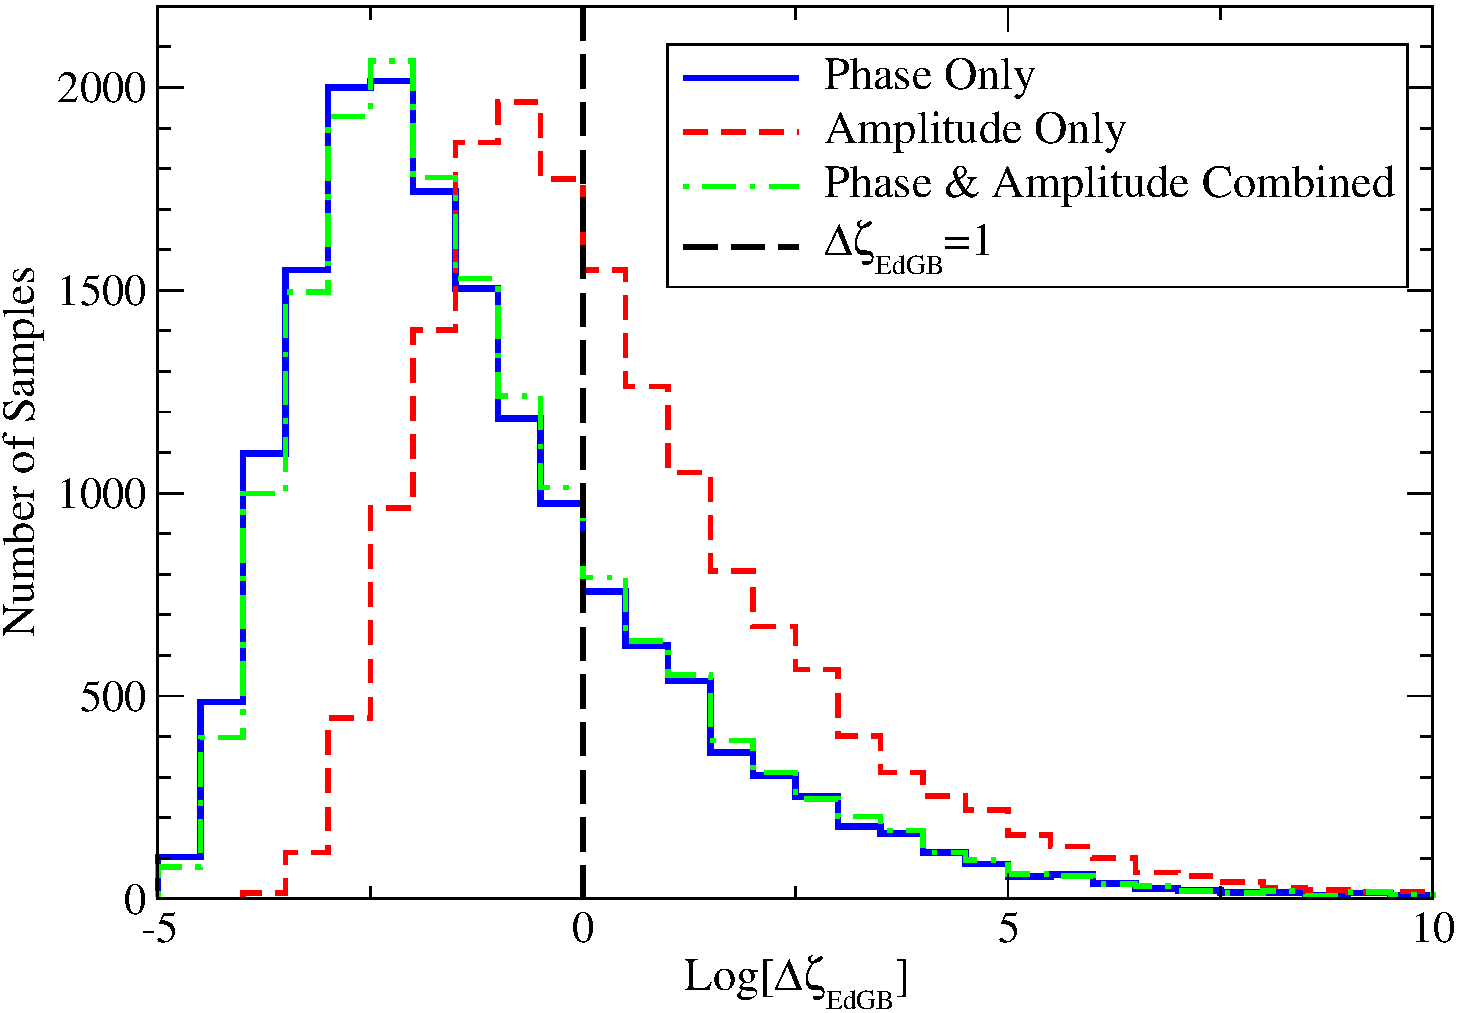
\includegraphics[width=8.5cm]{histogram-gw150914.pdf}
\caption{Histogram distributions of the 90\% CL bounds on $\zeta_{\EDGB}$ from a Fisher analysis with the phase correction only (blue solid), the amplitude correction only (red dashed) and combining the two corrections (green dotted-dashed). Fiducial values are taken from the posterior samples of GW150914. The samples that lie on the left side of the vertical black dashed line satisfy the small coupling approximation with 90\% CL.}
\label{fig:histogram-edgb}
\end{figure}


%Small coupling approximation
We now derive constraints on EdGB gravity from GW150914 and GW151226. First we estimate how well those events satisfy the small coupling approximation $\zeta_{\EDGB}<1$. To do so, we extract the 90\% CL upper bound $\Delta\zeta_{\EDGB}$ from each sample of the posterior distribution of a particular event. We then create histograms with all the samples (see Fig.~\ref{fig:histogram-edgb}) and calculate the fraction satisfying $\Delta\zeta_{\EDGB}<1$.  For GW150914, 72\% (42\%) of the samples satisfy the small coupling approximation if $\Delta\zeta_{\EDGB}$ is derived from the phase (amplitude) correction, while 70\% of the posterior distribution satisfies such approximation if the phase and amplitude corrections are combined. A similar analysis with GW151226 gives 98\% and 87\% for the phase and amplitude corrections respectively while combining the two yields almost the same result as that of the phase-only case. Since the fraction of samples satisfying $\zeta_{\EDGB}<1$ is much higher for GW151226 than GW150914 due to a larger number of GW cycles and slower relative velocity of the binary constituents, the former event places more reliable constraints on EdGB gravity compared to the latter one.


\begin{figure}[htb]
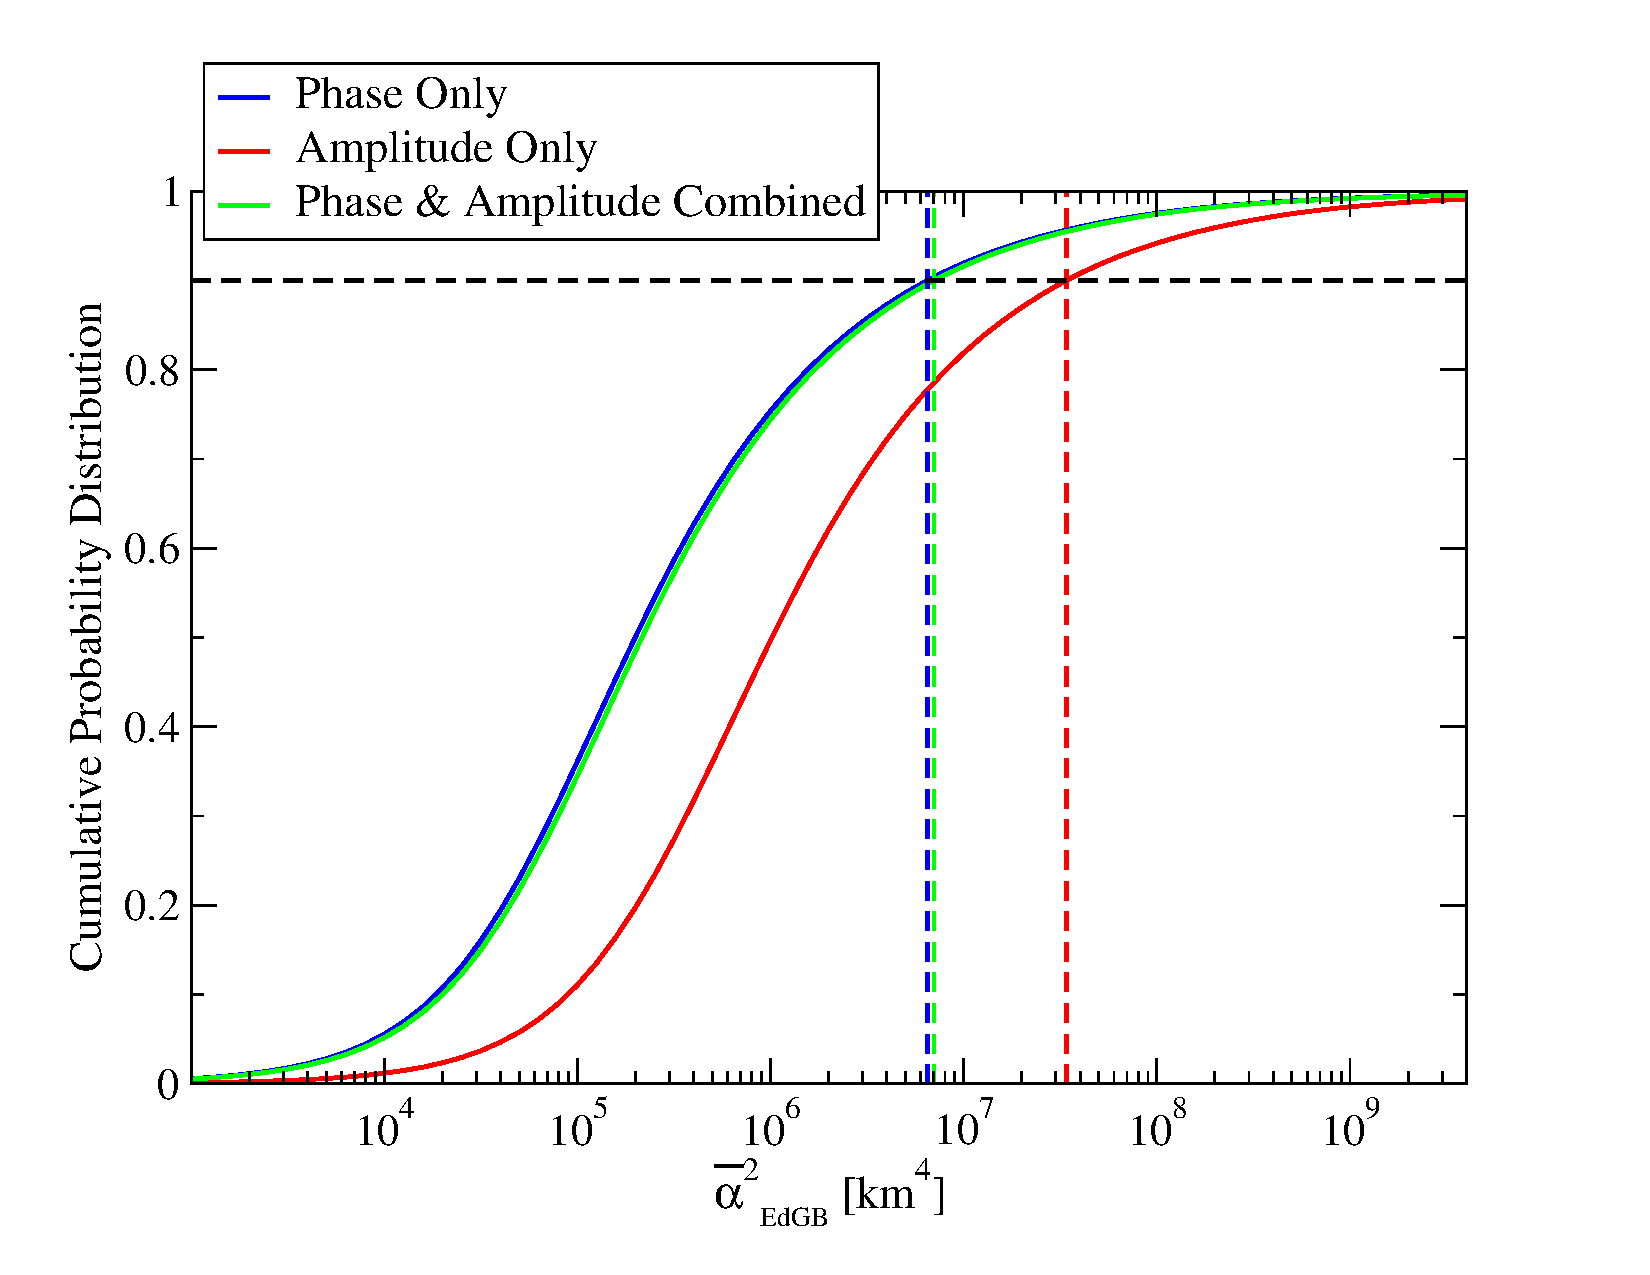
\includegraphics[width=8.5cm]{edgb-gw150914.pdf}
\caption{Cumulative probability distributions of $\bar{\alpha}^2_{\EDGB}$ obtained from GW150914 for the same three cases as in Fig.~\ref{fig:histogram-edgb}. Each vertical dashed line shows the corresponding 90\% CL upper bound of a solid line of the same color.}
\label{fig:pdf-edgb}
\end{figure}


%Results
Figure~\ref{fig:pdf-edgb} presents cumulative probability distributions of $\bar{\alpha}^2_{\EDGB}$\footnote{We show the distribution of $\bar{\alpha}^2_{\EDGB}$ instead of $\sqrt{\bar{\alpha}_{\EDGB}}$ as it is the former that directly enters in the waveform.} for GW150914 for three different cases with vertical lines showing the 90\% CL of the corresponding distribution. We found the 90\% CL constraints on  $\sqrt{\bar{\alpha}_{\EDGB}}$ from each of the phase and amplitude corrections as 50.5 km and 76.3 km respectively. Notice that these bounds have the same order of magnitude. On the other hand, combining the amplitude and phase corrections leads to an upper bound of 51.5 km, which is weaker than the  phase-only constraint by 2\%.
Similar analyses with GW151226 yield 4.3 km and 10.5 km respectively from th phase and amplitude corrections,
%\footnote{The upper bound on $\sqrt{\bar{\alpha}_{\EDGB}}$ derived from the phase correction with GW151226 agrees with those of ref.~\cite{Nair:2019iur} and~\cite{Yamada:2019zrb}}, 
while \kent{combining the two only changes the result from including only the phase correction by 0.01\%.} \sout{the difference between the phase-only case and the combined analysis  is only 0.01\%. As we can see,} 
These bounds are consistent with those in a recent paper~\cite{Nair:2019iur} while Ref.~\cite{Yamada:2019zrb} found even stronger bounds by combining multiple GW events. These GW bounds are comparable to the one obtained from low-mass X-ray binaries~\cite{Yagi:2012gp}.
Although GW150914 leads to weaker constraints on EdGB gravity compared to GW151226, the effect of amplitude correction is more manifest for the former event. \kent{This is because GW150914 has a smaller number of GW cycles and thus the amplitude contribution becomes relatively higher than GW151226.}

\ky{I added this paragraph.}
Why does the inclusion of the amplitude correction deteriorates the bound slightly from the case where one only includes the phase correction? This may sound counter-intuitive as one might think adding more EdGB corrections should improve the bound. Indeed, if one neglects correlations among $\bar \alpha^2_\EDGB$ and other binary parameters, addition of the amplitude correction improves the bound. However, such amplitude correction introduces a strong correlation between $\bar \alpha^2_\EDGB$ and the luminosity distance. As a result, the bound derived by including both the amplitude and phase corrections becomes weaker than that from the latter only.

\subsection{Scalar-Tensor Theories}


\subsection{Varying- $G$ Theories}

\section{Conclusion}
\section{Appendix}\label{Appendix}
%phenomB vs PhenomD for generation mechanism
%------------------------------------------------------- 
\bibliography{ppE}
\end{document}
